\chapter{Management Cases}

The following Use Cases show management features that are beneficial for Vertebra to emulate.  Some are couched in the example provided by another implementation.  Many of them are incomplete with respect to the full Vertebra ecosystem.  However, the core benefits of each one are embodied in Vertebra in one way or another.

There are also some Anti-Use Cases.  These provide management behaviors that we absolutely want to avoid.  You may notice that some technologies appear as a Use Case and an Anti-Use Case.  This is intentional, as often software that is good would be better without some of its baggage.

\section{Composition and Cascade}

One of the signs of a good data model is ``Don't Repeat Yourself'' (DRY\index[subject]{Agile Programming!DRY}\nomenclature{DRY}{literally ``Don't Repeat Yourself''; from agile programming, if the same data is entered in multiple places, it's generally taken to be a sign of a substandard model of the problem}).  If you have to record the same information in two different places (and it's not an optimization), then you have likely failed to model the data well.

DRY is a good rule of thumb for a programmer.  It's practically the \textbf{only} rule of thumb for an administrator.  If the administrator continually has to repeat himself, his job will rapidly scale out of control.  The use cases in this section are all written with that fact in mind.  Each of these cases identifies a decision to choose powerful ways to reduce and avoid repetition.

\subsection{Use Case: Composition of Permissions}

\paragraph{Description}

Permissions should be built holistically.  In the absence of permissions, we should be default-deny\index[subject]{permissions!default-deny}\nomenclature{Default-Deny}{in security, an absence of applicable permissions denies access to the secured object, analogous to \emph{strict construction} in legal systems}, an absence of sufficient permissions should be presumed to deny access to a secured entity.

Starting with this empty slate, permissions should be found that, in aggregate, allow an operation.  This is to mean that it operations are permitted by the composition\index[subject]{permissions!composition} of any assigned permissions, by the cascading\index[subject]{permissions!cascade} of permissions from ancestors, or possibly by compositions of those cascaded permissions.

Cascading permissions\index[subject]{permissions!cascade} should preserve the information about these relationships.  Thus, the cascade should be computed at the time of access, not at the time of assignment.

\paragraph{Discussion}

Starting with the abstract concept of a security entity, we can build a simple model for representing permissions.  We shall not differentiate an entity which initiates an operation from an entity upon which the operation is initiated.  This is largely because such entities may trade places at any time and, as such, any distinction would be meaningless.

Our security entities can be thought of as inheritance hierarchies.  These hierarchies should allow multiple inheritance, thus they are technically directed-acyclic-graphs, rather than a strict hierarchy or tree.

Depending on the semantics of the relationship, we may think of descendants in the hierarchy as being of some ``sub-type'' of the ``types'' represented by their ancestors or as being ``members'' of the ``groups'' represented by their ancestors.  In either case, they may be treated the same, and any terminology is only a handy tool for discussion, not an abstract constraint on the security model.

\paragraph{Example}

\begin{figure}[t]
	\begin{center}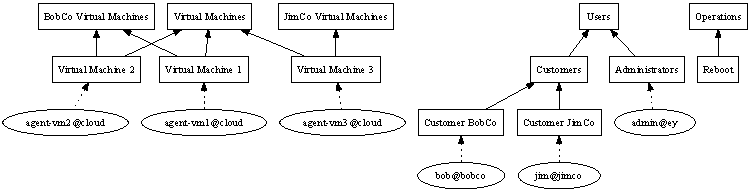
\includegraphics[width=\myfigwidth,height=\myfigheight,keepaspectratio]{figs/dot/bobco1}\end{center}
	\caption[Example Security Entities]{Sample Security Entities: BobCo and JimCo}\label{fig:bobco1-sec}
\end{figure}
\begin{table}[b]
	\begin{center}
		\begin{tabular}{| c | l | l |}
			\hline
				\multicolumn{3}{|c|}{Permissions} \\
			\hline
				\# & Source Entity & Destination Entity \\
			\hline \hline
				1 & Users & Reboot \\
			\hline
				2 & Administrators & Virtual Machines \\
			\hline
				3 & Administrators & Operations \\
			\hline
				4 & Customer BobCo & BobCo Virtual Machines \\
			\hline
				5 & Customer JimCo & JimCo Virtual Machines \\
			\hline
		\end{tabular}
	\end{center}
	\caption{Sample Permissions}
	\label{tbl:bobco1-perm}
\end{table}

An example diagram of a set of related objects is given in figure \ref{fig:bobco1-sec}.  Rectangles indicate abstract security entities. Ellipses mark concrete security entities. Dotted lines show association of the two.  A set of permissions on this model are shown in table \ref{tbl:bobco1-perm}.

The policy specified here is very powerful. \underline{Users} are allowed to \textsf{Reboot}.  \underline{Administrators} (and thus \emph{admin@ey}) are given the access to \underline{Virtual Machines} (i.e. \emph{agent-vm1@cloud}, \emph{agent-vm2@cloud}, \emph{agent-vm3@cloud}).  \underline{BobCo} and \underline{JimCo} are given access to just their respective machines.

If \emph{bob@bobco} were to attempt to issue an operation of the form \textsf{Reboot(Virtual Machine 1)}, permissions 1 and 4 combine to allow the operation.  Specifically, since \emph{bob@bobco} is a descendant of \underline{Users}, permission 1 applies.  Since \emph{bob@bobco} is a descendant of \underline{BobCo}, permission 4 applies.

If \emph{bob@bobco} were to attempt to issue an operation of the form \textsf{Reboot(Virtual Machine 3)}, no combination of permissions allow this.

If \emph{admin@ey} were to attempt to reboot any machine, permissions 1, 2, and 3 would combine.  Note that permission 1 is obviated by permission 3, but either would apply.

What is most interesting about this model, is the flexibility with which new virtual machines can be added, new users added, old users removed, new administrators added, et cetera.  At each point, no more work must be done other than to associate them with their respective abstract entity, and all permissions are applied.

This serves to help separate policy from permissions, which is absolutely critical in larger systems.

Another important feature that is not obvious from this example is that it is possible to allow someone to have two roles (i.e. inheritable permissions groups) with conflicting duties, but to prevent them from exercising their permissions simultaneously.  Assume, that we added a consultant who could operate on virtual machines for both BobCo and JimCo.  With a simple restriction, it is possible to only allow that consultant to activate one set of permissions or the other at a given time.

In addition these dynamic extensions, other rich extensions can be defined.  Examples include time-based limitations or static limitations (i.e. no one can ever be provisioned with a certain conflict being permitted).  These allow further specification of policy with a minimum of management.  Whether these extensions will ever be implemented in Vertebra is currently undecided, but an exciting possibility nonetheless.

\paragraph{Related Implementations}

\begin{itemize}
	\item Novell Netware\texttrademark\index[tech]{Novell\texttrademark!Netware\texttrademark}
\end{itemize}

\subsection{Anti-Use Case: Direct Permissions}

\paragraph{Description}

Permissions are assigned to users directly, or possibly to simple groups.  Objects are secured by some list of users and groups.

\paragraph{Discussion}

With perhaps the exception of a systems lacking a model of security, this is probably the most common model in large scale deployment.  While it can be functional, there are security concerns that cannot be addressed in this model.

The primary useful one is called ``Dynamic Separation of Duty''\index[subject]{permissions!dynamic separation of duty}.  Specifically, a situation can exist where there is a conflict of interest if a person has two permissions at the same time.

Consider a bank.  It is possible for a person to be a teller at a bank.  In some (likely most) cases, that teller may also be a customer of the bank.  It is a grave conflict of interest for a person to be a teller and also handle their own withdrawal or deposit.  This is because the teller is responsible for verifying the integrity of those transactions.  It is a long understood fact that avoiding situations where a person must protect their own interests and business interests is a prudent business practice.

With static permissions, there is not a good way to represent such constraints.  Some people compensate by creating multiple user accounts for a person.  However, this makes management much more complex, since administrators must ensure that these rules are followed, audit that they are maintained correctly, and manage many more user accounts doing so.

\paragraph{Example}

\begin{figure}[t]
	\begin{center}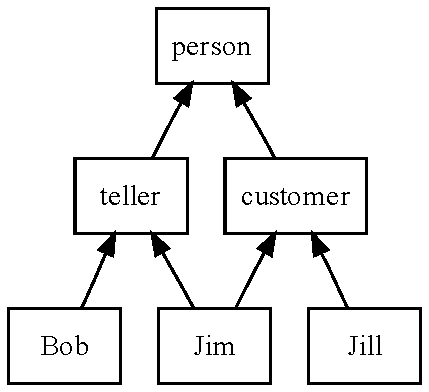
\includegraphics[width=\myfigwidth,height=\myfigheight,keepaspectratio]{figs/dot/bank_model}\end{center}
	\caption{Bank Example Model}\label{fig:perm-flat}
\end{figure}

Since this is an Anti-Use Case, we will demonstrate the pathological behavior described above.  A diagram of the model is in \ref{fig:perm-flat}.

In this particular case, there is no combination of permissions that can allow Jim, who is both a customer and a teller, to function both as a customer and a teller without enabling him to process his own transactions, which is a clear conflict of interest.

\paragraph{Related Implementations}

\begin{itemize}
	\item Microsoft Windows\texttrademark NTFS\index[tech]{Microsoft Windows\texttrademark!NTFS}
	\item Unix\texttrademark\index[tech]{Unix\texttrademark}
\end{itemize}

\subsection{Use Case: Cascading Configuration}

\paragraph{Description}

{\Large TODO:} Just like permissions, configuration can come from above.

paragraph{Discussion}

{\Large TODO}

\paragraph{Example}

{\Large TODO}

\paragraph{Related Implementations}

\begin{itemize}
	\item World Wide Web Consortium (W3C) Cascading Style Sheets\index[tech]{W3C!Cascading Style Sheets}
\end{itemize}

\subsection{Anti-Use Case: Lattice Configuration}

\paragraph{Description}

{\Large TODO:} A matrix of boxes, all ugly.  Let the computer do the work.

paragraph{Discussion}

{\Large TODO}

\paragraph{Example}

{\Large TODO}

\paragraph{Related Implementations}

{\Large TODO}

\section{Lessons From A Print Queue}

\subsection{Use Case: Job Enumeration}

\paragraph{Description}

{\Large TODO:} What's running is important, eh?

paragraph{Discussion}

{\Large TODO}

\paragraph{Example}

{\Large TODO}

\paragraph{Related Implementations}

{\Large TODO}

\subsection{Use Case: Job Management}

\paragraph{Description}

{\Large TODO:} If it runs, kill it!  Or pause it!  Or send some other exciting event toward it.

paragraph{Discussion}

{\Large TODO}

\paragraph{Example}

{\Large TODO}

\paragraph{Related Implementations}

{\Large TODO}

\subsection{Anti-Use Case: The 500 lb. Bomb}

\paragraph{Description}

{\Large TODO:} Try to kill job.  Job just won't die until completion.  Badness.

paragraph{Discussion}

{\Large TODO}

\paragraph{Example}

{\Large TODO}

\paragraph{Related Implementations}

{\Large TODO}

\subsection{Anti-Use Case: The Job That Wouldn't Die}

\paragraph{Description}

{\Large TODO:} Rather than waiting until completion, this job just hangs forever.  Also sucks.

paragraph{Discussion}

{\Large TODO}

\paragraph{Example}

{\Large TODO}

\paragraph{Related Implementations}

{\Large TODO}

\section{Forensics, Records, and Other Administrivia}

\subsection{Use Case: Distributed Logging}

\paragraph{Description}

{\Large TODO:} Spread Out The Love.

\paragraph{Example}

{\Large TODO}

\paragraph{Related Implementations}

{\Large TODO}

\subsection{Use Case: Meaningful Logs}

\paragraph{Description}

{\Large TODO:} Useful tagging and severity.

paragraph{Discussion}

{\Large TODO}

\paragraph{Example}

{\Large TODO}

\paragraph{Related Implementations}

\begin{itemize}
	\item Unix\texttrademark\index[tech]{Unix\texttrademark} syslog\index[tech]{Unix\texttrademark!syslog}
\end{itemize}

\subsection{Anti-Use Case: Central Logging}

\paragraph{Description}

{\Large TODO:} Log shipping is bad.

paragraph{Discussion}

{\Large TODO}

\paragraph{Example}

{\Large TODO}

\paragraph{Related Implementations}

{\Large TODO}

\subsection{Use Case: Log Querying}

\paragraph{Description}

{\Large TODO:} Using a tool to report on the logs is okay.  Querying logs scales much better than ``reading'' logs.  Seems like the same thing, but it's not.

paragraph{Discussion}

{\Large TODO}

\paragraph{Example}

{\Large TODO}

\paragraph{Related Implementations}

\begin{itemize}
	\item Erlang\index[tech]{Erlang} \textsf{log\_mf\_h}\index[tech]{Erlang!log\textunderscore mf\textunderscore h}
	\item Erlang\index[tech]{Erlang} Report Browser\index[tech]{Erlang!Report Browser}
\end{itemize}

\subsection{Anti-Use Case: Lossy, Insecure Logs}

\paragraph{Description}

{\Large TODO:} No security.  Lossy delivery.  Not distributed.

paragraph{Discussion}

{\Large TODO}

\paragraph{Example}

{\Large TODO}

\paragraph{Related Implementations}

\begin{itemize}
	\item Unix\texttrademark Syslog\index[tech]{Unix\texttrademark!syslog}
\end{itemize}

\subsection{Anti-Use Case: Inextensible Log}

\paragraph{Description}

{\Large TODO:} Binary format is nuts. Requires compiled code to extend log message types.

paragraph{Discussion}

{\Large TODO}

\paragraph{Example}

{\Large TODO}

\paragraph{Related Implementations}

Microsoft Windows\texttrademark Event Log\index[tech]{Microsoft Windows\texttrademark!Event Log}

\subsection{Use Case: Distributed Auditing}

\paragraph{Description}

{\Large TODO:} Helps diagnose catastrophes.  Also reduces trust-spread for audit log.  No intermediate can tamper with the audit logs because you always get them from the source.  Also handy because we get both sides of the story, which can be reconciled to detect lies.

paragraph{Discussion}

{\Large TODO}

\paragraph{Example}

{\Large TODO}

\paragraph{Related Implementations}

{\Large TODO}

\subsection{Anti-Use Case: Inextensible Audit Log}

\paragraph{Description}

{\Large TODO:} Limited audit events. Not distributed. One place to tamper. Difficult to query. Requires compiled code to extend audit message types.

paragraph{Discussion}

{\Large TODO}

\paragraph{Example}

{\Large TODO}

\paragraph{Related Implementations}

\begin{itemize}
	\item Microsoft Windows\texttrademark Audit Log\index[tech]{Microsoft Windows\texttrademark!Audit Log}
\end{itemize}
